\documentclass{beamer}
%
% Choose how your presentation looks.
%
% For more themes, color themes and font themes, see:
% http://deic.uab.es/~iblanes/beamer_gallery/index_by_theme.html
%
\mode<presentation>
{
  \usetheme{Madrid}      % or try Darmstadt, Madrid, Warsaw, ...
  \usecolortheme{beaver} % or try albatross, beaver, crane, ...
  \usefonttheme{default}  % or try serif, structurebold, ...
  \setbeamertemplate{navigation symbols}{}
  \setbeamertemplate{caption}[numbered]
} 

\usepackage[english]{babel}
\usepackage[utf8x]{inputenc}

\title[CCTC]{Classification of Crowdsourced Text Correction}
\author{Megha Gupta,
Dr. Haimonti Dutta (Advisor)}
\institute{Second Year Annual Presentation, 2013-2014 \\
IIIT Delhi}
\date{18-September-2015}
\begin{document}

\begin{frame}
  \titlepage
\end{frame}

\begin{frame}{Outline}
  \tableofcontents
\end{frame}

\section{Courses and TA duties}
\begin{frame}{Courses and TA duties}
\begin{itemize}
\item Courses (SGPA: 6, CGPA: 7.4) \\
MTH 505 - Linear Optimization (4 credits)
\item TA duties \\
CSE 561 - Probabilistic Graphical Modelling by Chetan Arora
\end{itemize}
\end{frame}

\section{Conferences and Workshops}
\begin{frame}{Conferences and Workshops}
Conferences
\begin{itemize}
\item Presented in ACM India SIGKDD Conference on Data Sciences, Banglore (IKDD CODS, 2015)
\item Attended the 3rd International Conference on Big Data Analytics at IIT Delhi (BDA, 2014)
\end{itemize}
\end{frame}


\section{Motivation}
\begin{frame}{Motivation}
\begin{itemize}
\item<1-> More than 200 million paper books are being published every year.
\item<2-> Ebooks require less storage, shared online, digitally processed, searched, translated, edited and annotated.
\item<3-> OCR results depend on factors like input paper quality, column layout, font sizes and style.
\item<4-> System answers to questions like, ``What different kinds of corrections are done by users ?" or ``What are the most common mistakes made by the OCR device ?".
\end{itemize}
\begin{block}<3->{Note}
OCR is the process of transforming typewritten text into machine-readable text and it is far from perfect.
\end{block}
\end{frame}

\section{Problem}
\begin{frame}{Problem}
To build a system for Classification of Crowdsourced Text Correction which takes input as log files containing garbled and manually corrected OCR text, parses and tokenizes them and builds models to categorize the corrections using state-of- the-art machine learning algorithms.
\end{frame}


\section{Architecture of the Proposed System}
\begin{frame}{Architecture of the Proposed System}
\begin{columns}
\column{.98\textwidth}
\begin{figure}[ht]
\begin{center}
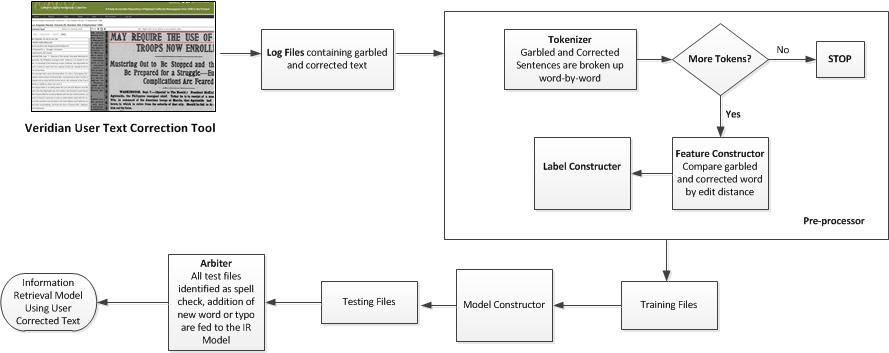
\includegraphics[height=1.7 in]{images/archOCR.jpg}
\end{center}
\end{figure}
\end{columns}
\end{frame}

%\section{Text correction tool}
\begin{frame}{Text Correction Tool}
%\begin{itemize}
%\item{Raw OCR text: }
\begin{columns}
\column{0.98\textwidth}
\begin{figure}[ht]
\begin{center}
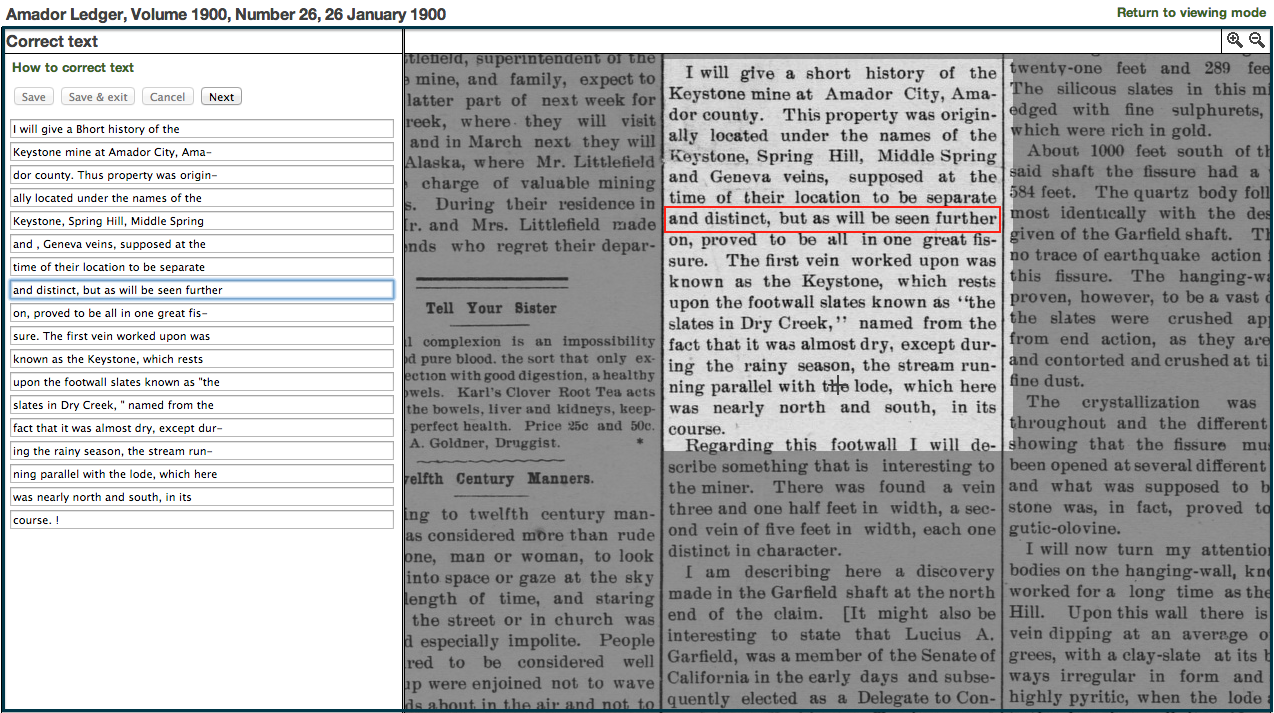
\includegraphics[height=2.5 in]{images/correction.jpg}
\footnote{http://veridiansoftware.com/crowdsourcing/}
\end{center}
\end{figure}
\end{columns}
\end{frame}


\begin{frame}{Datasets \footnote{https://github.com/megha89/}}
\begin{itemize}
\item Raw OCR text (Input)
\item Logfiles (Input)
\item Corrected OCR Text (Obtained)
\end{itemize}
\end{frame}

%\begin{frame}{Datasets: Corrected OCR text}
%\end{frame}

\section{Methodology}
\begin{frame}{Methodology}
\begin{itemize}
\item<1-> Tokenizer
\item<2-> Feature Constructor
	\begin{enumerate}
	\item Word-level Feature Construction (Proposed)
	\item Character-level Feature Construction (Baseline)
	\end{enumerate}
\item<3-> Label Constructor
	\begin{enumerate}
	\item Addition 
	\item Deletion
	\item Punctuation
	\item Capitalization
	\item Spellcheck
	\end{enumerate}
\item<4-> Model Construction : Joachim's Multiclass SVM
\item<5-> Information Retrieval Techniques

\end{itemize}
\end{frame}

\section{Results}
\begin{frame}{Results}
Table 1 and Table 2 show the Average Loss Error and Average Time taken by the baseline and proposed method using linear and non linear kernels respectively.
\begin{columns}
\column{.98\textwidth}
\begin{figure}[ht]
\begin{center}
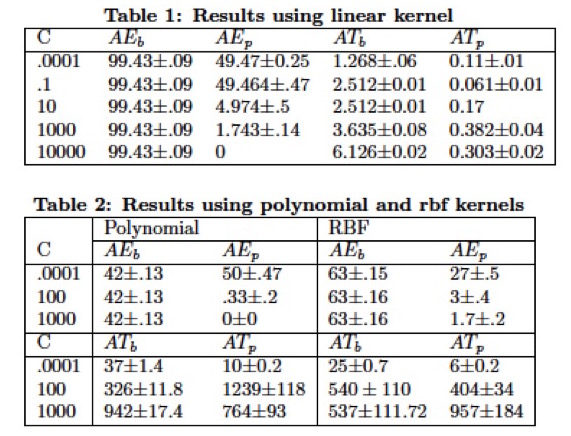
\includegraphics[height=2 in]{images/table.jpg}
\end{center}
\end{figure}
\end{columns}
\end{frame}


\begin{frame}{Results contd.}
\begin{columns}
\column{.98\textwidth}
\begin{figure}[ht]
\begin{center}
Examples of Capitalization Error, I --$>$ i
%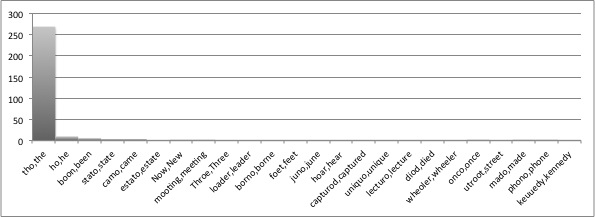
\includegraphics[height=1.5 in]{images/o_e.jpg}
%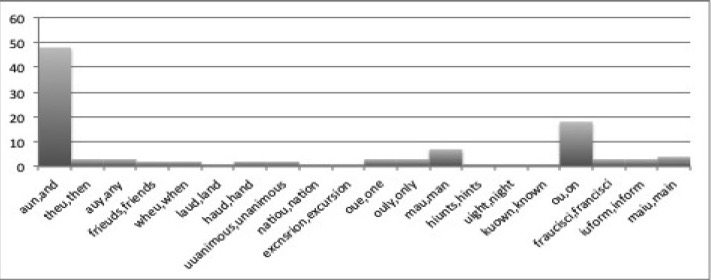
\includegraphics[height=1.5 in]{images/u_n.jpg}
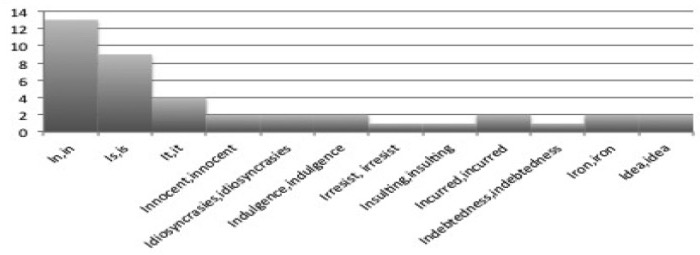
\includegraphics[height=1.5 in]{images/I_i.jpg}
\end{center}
\end{figure}
\end{columns}
\end{frame}

\section{Conclusion}
\begin{frame}{Conclusion}
\begin{itemize}
\item The manually crafted word-level features outperforms the automatically generated char-level features in terms of average loss error.
\item The non linear kernels performed better but the time taken by them was marginally high.
\end{itemize}
\end{frame}

\section{Future Work}
\begin{frame}{Future Work}
Though the manually crafted word-level dataset performed better but the time consumed was considerably higher, so there is a need to balance the tradeoff such that the algorithm becomes more compatible with the large scale datasets.
\end{frame}



\section{Ongoing Work}
\begin{frame}{Ongoing Work}
%Aggregate load forecasting \\
Problem: To perform aggregate load forecasting for disparate energy data sources using the ensemble based learning technique called Product of HMMs. \\

%Why PoHMMs ?
%
\begin{itemize}
\item<1-> Motivation
\begin{enumerate}
\item<2->  To avoid the unnecessary redundant information thus reducing the network traffic and improving the privacy of  the customers.
\item<3-> Efficient power system planning and operation, energy purchasing and generation, load switching and infrastructure development. 
\item<4-> Various factors that effect load forecasting are time factors, weather conditions, class of customers, special events, electricity price, fluctuating demand and supply.

\end{enumerate}
\item<4-> Dataset: REDD\footnote{http://redd.csail.mit.edu/}, IIITD Faculty Housing, Enernoc dataset \footnote{http://open.enernoc.com/data/}.

\end{itemize}
\end{frame}

\begin{frame}{Approach}
\begin{itemize}
\item Load forecasting at utility level is done in 3 ways:
\begin{enumerate}
\item completely aggregated
\item completely disaggregated
\item clustering based approach
\end{enumerate}
\item PoHMMs is a model that combines several HMMs by multiplying their individual distributions together and then renormalizing them.
\end{itemize}
\begin{center}
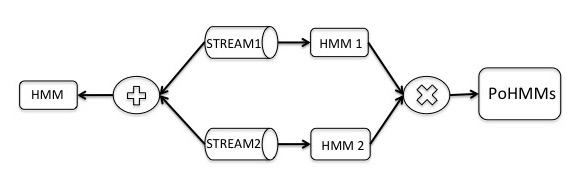
\includegraphics[height=1 in]{images/chart.jpg}
\end{center}
\end{frame}

\begin{frame}
\begin{itemize}
\item Figure below shows two HMMs $S^1$ and $S^2$ generated by two different data streams, the aggregate energy consumption can be modelled using PoHMMs as shown below.
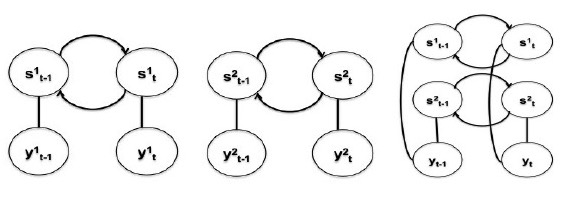
\includegraphics[height=1 in]{images/pohmm.jpg}
\end{itemize}
\end{frame}

\begin{frame}{Results}
Performance comparison between REDD, FH and Enernoc datasets is shown below.
\begin{center}
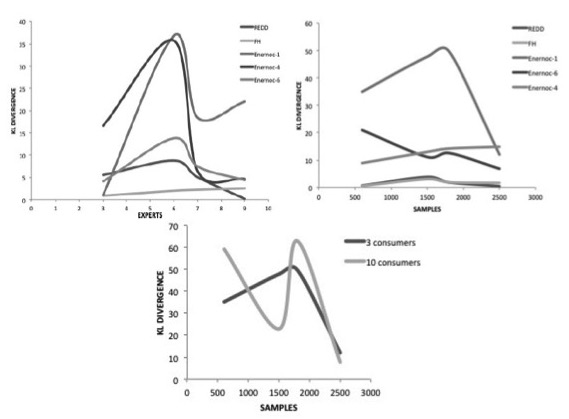
\includegraphics[height=2.5 in]{images/pohmm_res.jpg}
\end{center}
\end{frame}

\begin{frame}{Background Study}
TREC CDS Task\\
Problem: To retrieve the full biomedical articles that are relevant for answering generic clinical questions (``test",``diagnosis",``treatment") about medical records.



\end{frame}

%\vskip 1cm
%
%\begin{block}{Examples}
%Some examples of commonly used commands and features are included, to help you get started.
%\end{block}

%\bibliographystyle{abbrv}
%\bibliography{sigproc-sp}

\begin{frame}
    {\footnotesize
    \bibliographystyle{authortitle1}
    \bibliography{TEST}
    }
\end{frame}

\begin{frame}
\begin{center}
Thanks \\
Questions?
\end{center}
\end{frame}

\end{document}

